\documentclass[journal]{IEEEtran}
\usepackage{cite}

\usepackage{hyperref}
\usepackage[pdftex]{graphicx}
\usepackage{subfigure}
\usepackage{mathrsfs,amsmath}   %The amsmath package is included for \xrightarrow

\hypersetup{
	colorlinks=false,
	pdfborder={0 0 0},
}

\begin{document}
\title{Tumour Classification By Volumetric Image Analysis}
\author{
	\IEEEauthorblockN{Ashley J. Robinson\\}
	\IEEEauthorblockA{	University of Southampton\\
	\href{mailto:ajr2g10@ecs.soton.ac.uk}{ajr2g10@ecs.soton.ac.uk}
	}	
}


% The paper headers
\markboth{COMP6033: Independent Research Review. }	%	$27$/$03$/$14$.	DRAFT REPORT.}%
{Robinson: Effective Tumour Classification Exploiting Volumetric Image Analysis}

\maketitle


\begin{abstract}

This research review covers techniques available for the classification of tumours in the human body considering practical implications and stage interfacing.   
An architecture is proposed that follows basic image processing conventions but with an additional sub-module that provides non-technical confidence informations for a domain expert.  
The purpose of which is to classify tumours contained in medical images.
All image processing stages are considered only for the case of volumetric images.
Using a third dimension scales up complexity because of the amount of data available but has the potential to yield better results than a 2D approach.
Common techniques are reviewed and a selection is made on how to populate the architecture.
Human supervised deployment is considered whether stand-alone or as an extension to existing medical review software.

\end{abstract}







%\begin{IEEEkeywords}
%Tumour, Classification
%\end{IEEEkeywords}



\IEEEpeerreviewmaketitle







\section{Introduction}
\IEEEPARstart{T}{his} research review covers the use of volumetric image analysis in medicine to accurately classify tumours. 
The problem is to be approached by considering only the general case where no specific area of the human body is considered.
Rather than trying to classify lung or brain tumours individually the goal is to consider what tumours have in common and given an entire image of a human body is it possible to classify tumours in any given section?
The motivation behind this is to make the most of medical scanning.
Dosages of radiation, cost and simply the time required are all reasons to reduce the number of scans needed.
Making the most of any data gathered is a constructive method of scan frequency reduction.
The objective is to provide a recommendation for a system to be implemented such that a medical practitioner could use it as a tool for diagnosis.  

The architecture in Fig.~\ref{fig:Proposed} is the framework of the system to be recommended; inspired by those discussed in~\cite{ahmed2011efficacy,kumar2011classification,sachdeva2011multiclass,kostis03three}.
A chain of stages leads from raw data gathered from the patient to a diagnosis from a classification algorithm.
A confidence sub-block enables the domain expert to view the performance of the entire system without knowing the intricacies of operation; this requires processing to be explained with respect to their domain.
In medicine a threshold has to be selected carefully as false negatives in diagnosis are unjustifiable.

Raw data is captured from the patient and passed to system for pre-processing then feature extraction.
Input patterns are produced dependent on a pre-determined list of known useful features. 
Feature reduction and normalisation is then used to frame the data as such to make the most of the classification algorithm.

\begin{figure}[!htb]
   \centering
   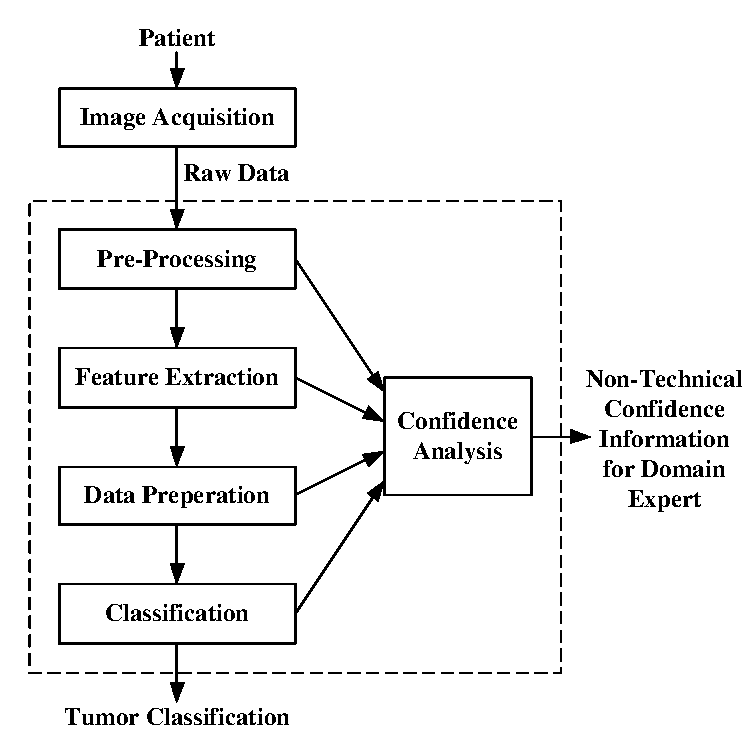
\includegraphics[width = 0.4\textwidth]{Figures/Proposed.pdf}
   \caption{Proposed system architecture.}
   \label{fig:Proposed}
\end{figure}











\section{Image Acquisition}
\label{sec:image}

A standard X-ray medical scan is tuned to produce and image of human bone.
The rays are attenuated by different materials in the body, more so by dense regions of bone, and the image is gained from this attenuation effect.  
This uses a single source and substrate to capture the image.
Taking multiple images from many different angles gathers more information and a 3D image can be made by stitching these together.
Fig.~\ref{fig:ct} describes the physical process of gathering data to be used in Computed Tomography (CT).
A ring allows images to be capture from 360$^{\circ}$ in a single plane then by moving in the orthogonal plane, in Fig.~\ref{fig:ct} through the paper, a full volumetric image of the patient can be made. 

\begin{figure}[!htb]
   \centering
   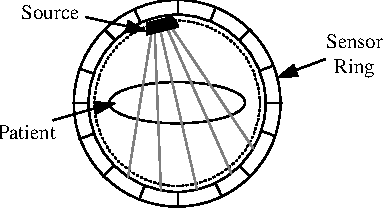
\includegraphics[width = 0.3\textwidth]{Figures/CT.pdf}
   \caption{Acquiring data from Computed Tomography. Adapted from~\cite{kayvan2006biomedical}.}
   \label{fig:ct}
\end{figure}

Any method of non-invasive image capturing in 2D can therefore be expanded to work in 3D by using the CT principle.
Different methods have tradeoffs such as radiation dosages and resolution.
Ultrasound is a method of image acquisition with the advantage of a small processing overhead allowing internal organs to be viewed in real-time which is beneficial because it allows practitioners to view internal physical movement. 
It can be used for CT but higher resolution methods are usually favoured such as X-ray and Magnetic Resonance Imaging (MRI).

There are also other non-intrusive methods that do not use electromagnetic or ultrasonic waves.
Hand palpitation is a common technique used by medical practitioners to gain an impression of abnormalities near the surface of the human body. 
Electromechanical apparatus employing the same technique can be used transfer the geometry of a growth to a volumetric image~\cite{liu09haptic,wellman1997modeling}.  
Only part of the area under inspection is visible so the technique has obvious drawbacks.

Data is typically stored as a series of greyscale 2D images which are slices of the scan.
The image viewer will build 3D images as and when required using these slices.
The common medical standard for these images is DICOM which holds the slices, relative position and also patient information~\cite{dicom11nema}.
Viewing the data naturally proves problematic because it is 3D data shown in an isometric fashion on a 2D screen.
Viewing software provides interactive images as shown in Fig.~\ref{fig:3d} which allows the user to move three slices to gain an impression of the region.

\begin{figure}[!htb]
   \centering
   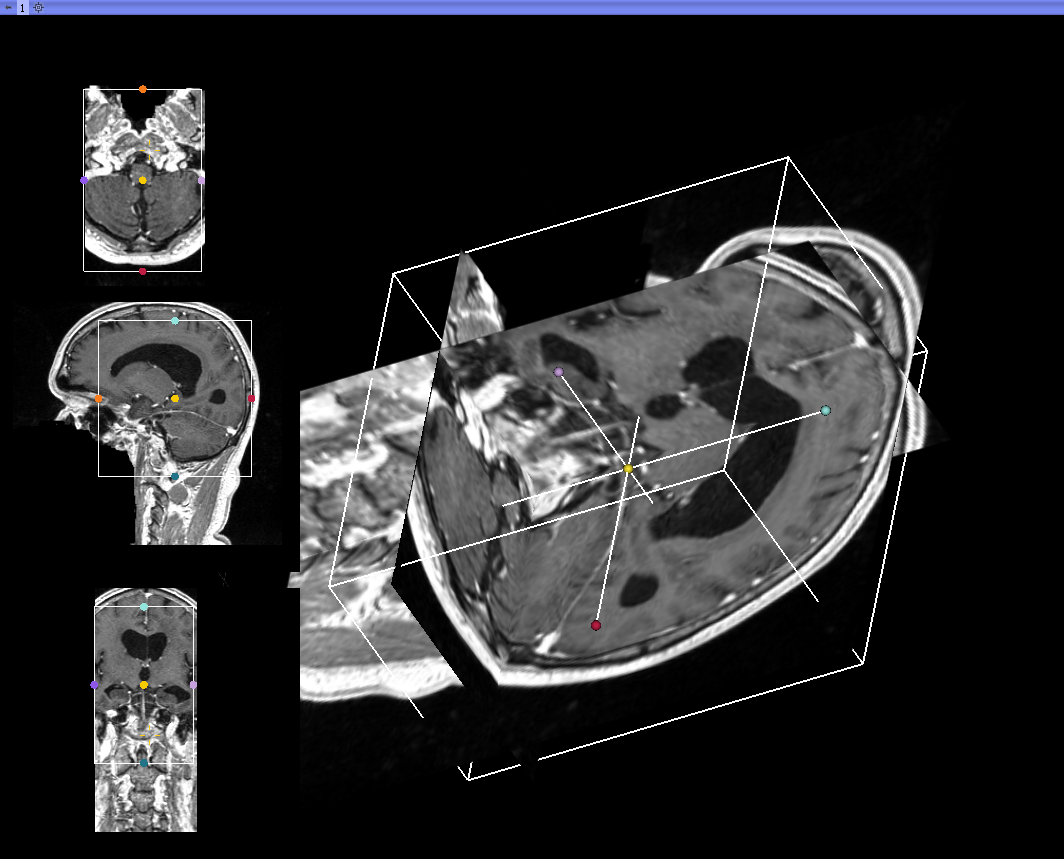
\includegraphics[width = 0.4\textwidth]{Figures/3Dview.png}
   \caption{An MRI scan of a healthy brain taken from~\cite{cia} and rendered by~\cite{slicer}.}
   \label{fig:3d}
\end{figure}

The analogue of a pixel (picture element) in 2D image is called a voxel (volumetric element) in a 3D image.
This is exactly the same idea but with a extra dimension to form a cube~\cite{lohmann1998volumetric}.
They can be considered cubes but also points which may make visualisation and processing easier to understand.
Fig.~\ref{fig:neighbourhood} describes how voxels are packed and three different neighbourhoods the can be considered when inspecting one voxel. 
Considering voxels to have larger neighbourhoods can increase the time complexity of some algorithms.


\begin{figure}
	\centering
	\subfigure[6]{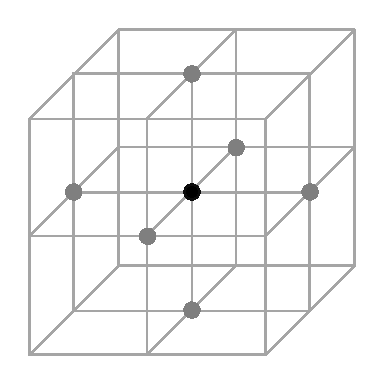
\includegraphics[width = 0.12\textwidth]{Figures/6N.pdf}
	\label{fig:neighbourhood6}}
	\subfigure[18]{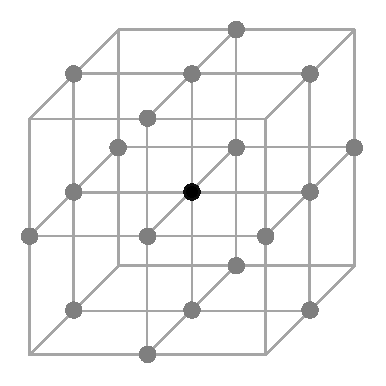
\includegraphics[width = 0.12\textwidth]{Figures/18N.pdf}
	\label{fig:neighbourhood18}}
	\subfigure[26]{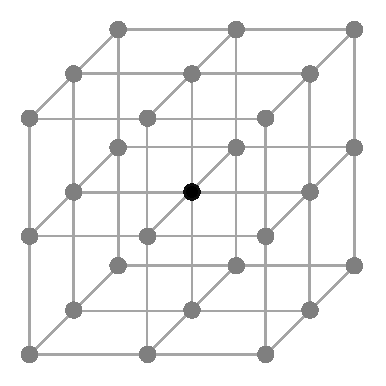
\includegraphics[width = 0.12\textwidth]{Figures/26N.pdf}
	\label{fig:neighbourhood26}}
\caption{Voxel Neighbourhoods~\cite{lohmann1998volumetric}.}
\label{fig:neighbourhood}
\end{figure}










\section{Pre-processing}
\label{sec:pre}

The provided raw data needs to be converted from the delivery format from the acquisition technology to a 3D matrix ready for generic processing.
Watermarking, which may have been inserted for human review, should also be removed at this stage. 
This is trivial in theory but requires a database of artefacts or manual review to accomplish.
There are also techniques, not considered in this paper, which can be applied just to the slices of a volumetric image which may be used to reduce processing overheads~\cite{harauz86exact}.

There are different techniques available to enhance the image captured or ensure it is correctly formatted for further processing.
This is considered as a mapping from an original image to a new image, $\textbf{I} \mapsto \textbf{I}'$, using only information from the original image.

\subsection{Histogram Operations}

An image histogram is a mapping from an image to a 2D plot of the frequency of voxel intensity; possible since voxels can have a discrete value of intensity within a fixed range.
This contains information on the type of material seen in the image, if it can be determined from intensity, and how much of that material is used to form the entire image.
Image enhancement can be performed using point operations with information from the histogram.
This is a very fast methods of image enhancement as it is direct voxel-to-voxel mapping; see Eq.~\ref{eqn:point}. 
Normalisation stretches the histogram to cover all available values of intensity therefore improving contrast.
Equalisation attempts to flatten the histogram by distributing intensity~\cite{nixon02feature}.

\begin{equation}
	I'(u,v,w) = \alpha(u,v,w)I(u,v,w)
	\label{eqn:point} 
\end{equation}



\subsection{Spatial Filtering}
Spatial filters use the neighbourhood of voxels to create a new value for each voxel in an image. 
The original image is mapped to a new image through a filter kernel, as described in Eq.~\ref{eqn:kernel}.
The filter kernel is a fixed dimension sub-image with a weighting on each voxel that is applied to every voxel in the original image.
This is spatial convolution.
If the filter kernel contains all ones it is known as a \emph{box filter} and performs smoothing on the image to remove noise.
A Gaussian filter performs better by placing a higher weighting on the central voxel and less on the extreme voxels~\cite{lohmann1998volumetric}.


\begin{equation}
	I'(u,v,w) = \sum\limits_{(i,j,k) \in R_H} I(u + i,v + j, w + k)H(i,j,k)
	\label{eqn:kernel} 
\end{equation}



\subsection{Frequency Filtering}
The Fourier transform, as used spatially on 2D images, can be extended to 3D images.
A Discrete Fourier Transform (DFT) for a $N$$\times$$N$$\times$$N$ voxel image is held in Eq.~\ref{eqn:dft}.
The spatial filtering process performs convolution so once an image is in the frequency domain the same effects can be achieved using multiplication.
It may prove more efficient to filter an image in the frequency domain rather than space if the required filter kernel is large.
Band-pass and notch filter operations can also be perform in the frequency domain.
Eq.~\eqref{eqn:same} provides the same result as Eq.~\eqref{eqn:kernel} using the increase transform implied from Eq.~\eqref{eqn:dft}. 

\begin{equation}
	F_{u,v,w} = \frac{1}{N^{\frac{3}{2}}} \sum\limits_{x=-\frac{N}{2}}^{\frac{N}{2}-1}\sum\limits_{y=-\frac{N}{2}}^{\frac{N}{2}-1}\sum\limits_{z=-\frac{N}{2}}^{\frac{N}{2}-1}I_{x,y,z}e^{-j\frac{2\pi}{N}(ux + vy + wz)}
	\label{eqn:dft} 
\end{equation}

%\begin{equation}
%	\textbf{F} = \mathcal{F}(\textbf{P}),\:\:\textbf{P} = \mathcal{F}^{-1}(\textbf{F}) 
%	\label{eqn:ft} 
%\end{equation}

\begin{equation}
	\textbf{I}' = \mathcal{F}^{-1}(\mathcal{F}(\textbf{I})*\mathcal{F}(\textbf{H}))	% Arrow doesn't work, implied matrices?
	\label{eqn:same} 
\end{equation}


\subsection{Additional Processes}
Anisotropic diffusion is a powerful technique used to enhance images.
The technique has been expanded from common 1D and 2D applications to 3D medical usage on MRI data~\cite{greig92nonlinear}.





\section{Feature Selection}
\label{sec:selection}
Before features can be extracted from a image it must be clear what features will be useful to a classification algorithm.
Reducing dimensionality through feature reduction can often prove more effective then lower dimensional projection methods; discussed in Section~\ref{sec:reduce}.
The recommendation of feature selection can come from domain knowledge or convergence on a subset that will provided a sufficiently low training error using an iterative tuning algorithm~\cite{bu07feature,li10tumor}.
A combination of both suits this purpose where domain knowledge may over recommend features and a machine learning approach can prune as required for the subset.  






TODO:


\begin{itemize}
  \item Review tumour features
  \item Attempt to generalise these features
\end{itemize}






\section{Feature Extraction}
\label{sec:extraction}


TODO:


\begin{itemize}
  \item Review different methods
  \item Recommend for this case
\end{itemize}






\section{Dimensionality Reduction}
\label{sec:reduce}





TODO:


\begin{itemize}
  \item Is this needed?
  \item Common techniques
  \item What fits with expected data
\end{itemize}









\section{Classification}
\label{sec:class}



TODO:


\begin{itemize}
  \item How the data will look
  \item Computational overheads
  \item Confidence output
\end{itemize}










\section{Conclusions}
\label{sec:conclusions}

It is clear that this tool can't be used as a hard and fast method of tumour diagnosis but instead as a valuable tool for image reviewers.
Software packages designed for medical image review, such as~\cite{slicer}, have bidirectional interfaces to custom extensions.
Implementing this system as an extension would remove many overheads required in data handling but reduce the scope for optimisation.
The feedback from the entire process would be a checklist which the user must manually review and waive if incorrectly identified. 










\bibliographystyle{ieeetran}
\bibliography{references}

\end{document}


